\documentclass{article}
\usepackage[english]{babel}
\usepackage[utf8]{inputenc}
\usepackage[T1]{fontenc}

\usepackage{amsmath} % math stuff
\usepackage{amssymb} % math stuff
\usepackage{amsthm}  % math stuff
\usepackage{commath} % math stuff
\usepackage{relsize} % math stuff
\usepackage{caption} % caption stuff
\usepackage{fancyhdr} % custom headers
\usepackage{lastpage} % determine last page for the footer
\usepackage{extramarks} % headers and footers
\usepackage{graphicx} % images
\usepackage{listings} % code listings
\usepackage{courier} % courier font
\usepackage{enumerate}
\usepackage{enumitem}
\usepackage{mathtools}
\usepackage{titling}
\usepackage{float}
\usepackage{cite}
\usepackage[mathscr]{eucal}
\usepackage{subcaption}
\usepackage{marvosym}
\usepackage{makecell}
\usepackage{hyperref}
\usepackage{multirow}
\usepackage{rotating}

\usepackage{pgfplots}
\pgfplotsset{
  every axis plot/.append style={line width=0.8pt},
  compat=1.17,
}

%tikz
\usepackage{tikz}
\usetikzlibrary{arrows}
\usetikzlibrary{positioning}

\newcommand{\given}{\,\middle|\,}
\def\arraystretch{1.3}

\title{Self-supervised improvements to model-based reinforcement learning with internal state representations}
\author{Julien Scholz}
\date{\today}

\begin{document}

\begin{titlepage}
    \centering
    University of Hamburg \par
    MIN Faculty \par
    Department of Informatics \par
    BSc Informatics \par
    \vspace{6\baselineskip}
    {\Large Bachelor's Thesis\par}
    {\Huge \thetitle \par}
    \vspace{6\baselineskip}
    by\par
    {\Large \theauthor \par 7065721 \par}
    \vfill
    Thesis advisors:\par
    {\large Dr. Cornelius Weber, \par Muhammad Burhan Hafez}
\end{titlepage}

\begin{abstract}
    \noindent
    Using a model of the environment, reinforcement learning agents can plan ahead and achieve super-human performance in board games like Chess, Shogi and Go, while remaining relatively sample efficient. As demonstrated by the MuZero Algorithm, the environment model may even be learned dynamically, generalizing the agent to many more tasks while achieving state-of-the-art performance. Notably, MuZero uses internal state representations instead of real environment states for its predictions. In this thesis, we introduce two additional, independent loss terms to MuZero's overall loss function, which work entirely unsupervised and act as constraints to stabilize the learning process. Experiments show that they provide a significant performance increase on simple OpenAI Gym environments. The modifications also enable self-supervised pretraining for MuZero, that is, the algorithm can learn about environment dynamics before a goal is made available.
\end{abstract}

\vfill

\renewcommand{\abstractname}{Zusammenfassung}
\begin{abstract}
    \noindent
    
\end{abstract}

\tableofcontents

\newpage

\begin{frame}{Getting robots bored enough to stack cubes}
    \begin{figure}
        \centering
        \includegraphics[width=0.5\textwidth]{assets/cube_stacking.png}
        \caption{A \textit{Dobot} robotic arm being tasked with picking up and stacking simulated cubes in \textit{CoppeliaSim}\footnote{\url{https://www.coppeliarobotics.com/}}.}
        \label{fig:cube_stacking}
    \end{figure}
\end{frame}

\begin{frame}{TODO}
    \begin{itemize}
        \item Reinforcement learning is difficult
        \item Google DeepMind's \textit{MuZero Algorithm} \cite{muzero} may need a team of experts (and supercomputers) to operate
        \item We set out to make MuZero more robust
    \end{itemize}
\end{frame}

\newpage
\section{Background}
\subsection{Reinforcement Learning}
\textit{Reinforcement learning} is the act of learning a mapping from \textit{observations} to \textit{actions} so as to maximize a real-valued \textit{reward}. In contrast to another learning paradigm, \textit{supervised learning}, the learner is not told which actions result in the largest reward for different observations. Instead, an agent must try out different actions in different situations to discover a useful behavior. \cite{sutton}

The principles behind reinforcement learning are inspired by the way animals learn. Behavioral psychology has found that actions can be encouraged or surpressed when they are followed up with positive or negative stimuli \cite{thorndike}.

\subsubsection{Markov Decision Process}
The interaction aforementioned interaction of a learner with its surroundings to achieve a goal can be modeled mathematically through a \textit{Markov Decision Process} (or \textit{MDP}) \cite{bible}. This enables us to prove statements concerning learning algorithms theoretically, such as the convergence of an agent's behavior to its optimum.

We start by defining that the learning and acting instance is called the \textit{agent}, whereas its surroundings, which deliver situations, respond to the agent's actions, and control the reward signal, are called the \textit{environment}. The agent, therefore, strives to maximize environment rewards by performing actions based on previously perceived situations in the environment. 

In Markov Decision Processes, the agent-environment interaction only occurs at discrete timesteps $t \in \{0, 1, 2, ...\}$. At each timestep $t$, the environment provides a \textit{state} $S_t \in \mathscr{S}$ to the agent, where $\mathscr{S}$ is the set of all possible states. Based on this state, the agent must select an \textit{action} $A_t \in \mathscr{A}(S_t)$, with $\mathscr{A}(S_t)$ being the set of legal actions in state $S_t$. As a result of this action, the agent receives a \textit{reward} $R_t \in \mathscr{R} \subset \mathbb{R}$ and progresses onwards to the next state $S_{t+1}$. Note that this means there is no reward associated with the very first timestep. A sequence following this pattern of states, actions, and rewards is called a \textit{trajectory}. This process is visualized in figure \ref{fig:mdp_visualization}.

\begin{figure}[ht]
    \centering
    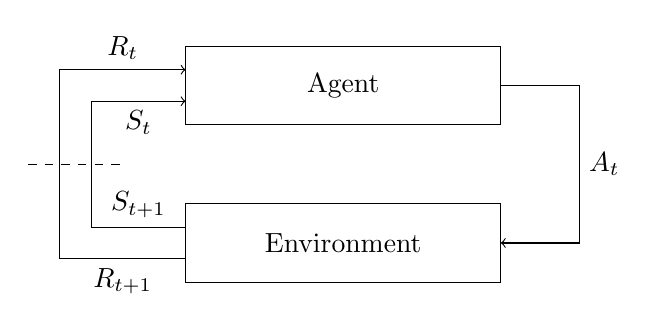
\begin{tikzpicture}
        \draw (0, 2) rectangle node {Agent} (4, 3);
        \draw (0, 0) rectangle node {Environment} (4, 1);

        \draw [->] (4, 2.5) -- (5, 2.5) -- node[right] {$A_t$} (5, 0.5) -- (4, 0.5);

        \draw [->] (0, 0.3) -- node[below] {$R_{t+1}$} (-1.6, 0.3) -- (-1.6, 2.7) --node[above] {$R_t$}  (0, 2.7);
        \draw [->] (0, 0.7) -- node[above] {$S_{t+1}$} (-1.2, 0.7) -- (-1.2, 2.3) -- node[below] {$S_t$} (0, 2.3);

        \draw [dashed] (-2, 1.5) -- (-0.8, 1.5);
    \end{tikzpicture}
    \caption{The agent-environment feedback loop in a Markov Decision Process.}
    \label{fig:mdp_visualization}
\end{figure}

In a \textit{finite Markov Decision Process} \cite{bible}, the sets of states $\mathscr{S}$, actions $\mathscr{A}(s) : \forall s \in \mathscr{S}$, and rewards $\mathscr{R}$ are all finite. With this constraint, we can create a function $p : \mathscr{S} \times \mathscr{R} \times \mathscr{S} \times \mathscr{A} \mapsto \left[0, 1\right]$ to denote probabilities of state transitions occurring. For example, $p\left(s', r \given s, a\right)$ refers to the probability of seeing state $s'$ and receiving reward $r$ after taking action $a$ in state $s$. This implies that transition probabilities are only dependent on the current state and action, but not on historical information.

Usually, an agent is not supposed to focus solely on choosing the action $A_t$ which results in the highest \textit{immediate reward} $R_{t+1}$. Instead, future rewards should also be taken into consideration. Formally, we define the \textit{return}, which is the sum of all rewards at subsequent timesteps until the final timestep $T$.
\begin{equation*}
    G_t = R_{t+1} + R_{t+2} + R_{t+3} + ... + R_T
\end{equation*}
Accordingly, an agent shall aim to maximize the expected return at each step. The concept of a final timestep only applies to tasks that have a clearly defined beginning and end, making them repetitive in nature. We call a single cycle of these repetitive tasks \textit{episode}.

For tasks that can potentially continue indefinitely, i.e. $T = \infty$, $G_t$ may also become infinite and can, therefore, no longer be subject to maximization. To avoid this issue, we introduce a \textit{discount rate} (or \textit{discount factor}) $\gamma \in [0, 1]$, and define the \textit{discounted return} as follows:
\begin{equation*}
    G_t^{(\gamma)} = R_{t+1} + \gamma R_{t+2} + \gamma^2 R_{t+3} + ...
        = \sum_{k=t+1}^T \gamma^{k-t-1} R_k
\end{equation*}
The parameter $\gamma$ determines to what extend the agent prefers rewards in the near over those in the far future. As an example, an agent with $\gamma = 0$ is only concerned with the immediate reward, whereas the same agent with $\gamma = 0.99$ will optimize for a large time window of rewards. Choosing $\gamma < 1$ ensures that $G_t$ will never become infinite.

In some cases, it is not realistic that the agent receives the full state of the environment. For instance, a robot with a camera cannot possibly measure all physical properties of its surroundings at all times. While a well defined \textit{latent state} may exist, the agent is only provided with an \textit{observation} produced by this state instead. These types of environments are modeled as \textit{Partially Observable Markov Decision Processes}, or \textit{POMDPs} \cite{bible}.
\subsubsection{Policy and Value Functions}
An agent's behavior can be described stochastically. We define the \textit{policy} of an agent to be the probability distributions for taking each available action in the respective states. For a state $s \in \mathscr{S}$, a legal action $a \in \mathscr{A}(s)$, and a policy $\pi$, $\pi\left(a \given s\right)$ is the probability that the agent will perform $a$ in $s$. The learning process consists of adapting $\pi$ over time to maximize the expected return \cite{bible}.

The \textit{value} is another useful measure for a reinforcement learning agent. It describes how good it is for the agent, following a specific policy, to be in a specific state. In other words, the value is the expected return for a policy. We define the \textit{state-value function for policy $\pi$} \cite{bible} as
\begin{equation*}
    v_\pi(s) = \mathbb{E}_\pi\left[G_t | S_t = s\right]
             = \mathbb{E}_\pi\left[\sum_{k=0}^\infty \gamma^k R_{t+k+1} \given S_t = s\right], \forall s \in \mathscr{S}
\end{equation*}
for Markov Decision Processes.

State-value functions do not apply to cases in which the agent tries to diverge from its current policy $\pi$. Because of this, we additionally define the \textit{action-value function for policy $\pi$} \cite{bible}, $q_\pi$, as the expected return when taking any action $a \in \mathscr{A}(s)$ in state $s \in \mathscr{S}$, and subsequently following policy $\pi$:
\begin{equation*}
    q_\pi(s, a) = \mathbb{E}_\pi\left[G_t | S_t = s, A_t = a\right]
             = \mathbb{E}_\pi\left[\sum_{k=0}^\infty \gamma^k R_{t+k+1} \given S_t = s, A_t = a\right], \forall s \in \mathscr{S}
\end{equation*}
\subsubsection{Policy-Based Methods}
We now explain one possible approach to optimize an agent's behavior by directly manipulating its parameterized policy $\pi_\theta$ with regards to the expected returns $\mathbb{E}\left[G_t\right]$. Typically, this is done using gradient descent. The REINFORCE algorithm \cite{reinforce} defines an estimate for $\nabla_\theta \mathbb{E}\left[G_t \given S_t \right]$ as $\nabla_\theta \log \pi_\theta\left(A_t \given S_t\right) G_t$, coining the term \textit{policy gradient}. Intuitively, this may be thought of as increasing or decreasing the probability of actions on a given trajectory based on the return of said trajectory.

Because the return of an entire trajectory needs to be determined before adjusting the policy, REINFORCE may, by itself, only be used in episodic tasks where training occurs at the end of an episode.

The regular is prone to high variance, which can slow down learning. A baseline can be introduced, which is shown to remain unbiased and often improves performance: $\nabla_\theta \log \pi_\theta\left(A_t \given S_t\right) \left(G_t - b(S_t)\right)$.
\subsubsection{Value-Based Methods}
In value-based methods, the agent maintains estimates of the state-value or action-value functions to improve its behavior. The key concept of value-based methods is the recursive definition for value functions, known as the \textit{Bellman equation} \cite{bible}:
\begin{align*}
    v_\pi &= \mathbb{E}_\pi \left[G_t \given S_t = s\right] \\
          &= \mathbb{E}_\pi \left[R_t + G_{t+1} \given S_t = s\right] \\
          &= \sum_a \pi\left(a \given s\right) \sum_{s'} \sum_r p\left(s', r \given s, a\right) \left[r + \gamma \mathbb{E}_\pi\left[G_{t+1} \given S_{t+1} = s'\right]\right] \\
          &= \sum_a \pi\left(a \given s\right) \sum_{s'} \sum_r p\left(s', r \given s, a\right) \left[r + \gamma v_\pi\left(s'\right)\right]
\end{align*}
Put into words, the value of a state is the sum of all possible immediate rewards and discounted values of subsequent states, weighted by their occurrence probabilities. A similar definition can be created for action-value functions:
\begin{equation*}
    q_\pi\left(s, a\right) = \sum_{s'} \sum_r p\left(s', r \given s, a\right) \left[r + \gamma q_\pi(s', a')\right]
\end{equation*}
The optimal policy $\pi^*$, given the correct action-value function $q_{\pi^*}$, would always perform the action with the highest $q$-value, i.e. the largest expected return. In turn, the action-values created by this policy are always the highest possible expected returns of any action. We find ourselves in a stable condition, known as the \textit{Bellman optimality equation} \cite{bible}, where $q_*$ denotes the action-value function for the optimal policy:
\begin{equation*}
    q_*\left(s, a\right) = \sum_{s'} \sum_r p\left(s', r \given s, a\right) \left[r + \gamma \max_{a'} q_*(s', a')\right]
\end{equation*}

In practice, the transition probabilities $p$ are usually not known. Q-learning \cite{q-learning} approaches this issue by iteratively updating a $q$-value estimates (which we will refer to as $Q$) in a tabular form, known as the Q-table. The iterative formula
\begin{equation*}
    Q\left(S_t, A_t\right) \gets Q\left(S_t, A_t\right) + \beta\left(R_{t+1} + \gamma \max_a Q\left(S_{t+1}, A_t\right) - Q\left(S_t, A_t\right)\right),
\end{equation*}
where $\beta$ is the learning rate hyperparameter, closely resembles the Bellman optimality equation. We are updating the current value estimate from the $Q$-table entry using the acquired information $R_{t+1}$ as well as a future, \textit{bootstrapped} value estimate $\max_a Q\left(S_{t+1}, A_t\right)$. This form of learning from future estimates is referred to as \textit{temporal-difference learning} or \textit{TD learning} \cite{td-learning}. The difference between the current estimate and the bootstrapped estimated combined with new experience is called the \textit{TD error}.

Note that Q-learning, similarly to other value-based methods, requires discrete, finite actions, whereas the aforementioned REINFORCE algorithm is capable of handling continuous action spaces. To define a Q-table, the number of possible environment states must also be finite and relatively small, which makes visual tasks virtually impossible. However, unlike REINFORCE, Q-learning is an \mbox{\textit{online}} algorithm \cite{bible}, meaning it can learn from data as soon as it is available (while interacting with the environment), and does not need to wait for the end of an episode. Thus, it can also be used for non-terminating tasks.
\subsubsection{Actor-Critic Methods}
\subsection{Artificial Neural Networks}
\textit{Artificial neural networks} (\textit{ANNs}), sometimes referred to as \textit{neural networks} (\textit{NNs}), are a category of bio-inspired algorithms that are structured like and can learn similarly to a brain. They are the foundation to many modern machine learning systems. Early concepts have been developed in 1943 \cite{first-neuron}, but they were not widely applicable due to the lack of computational resources. However, today, even consumer grade graphics cards intended for video games are powerful enough to run complex neural network models and are starting to be engineered specifically to accelerate machine learning applications \cite{tensor-cores}.

At their core, artificial neural networks are function approximators. Say, for example, we want to predict the output of a function $g$ without knowledge of its inner workings. Instead, we are only given several input-output samples produced by $g$. In this case, we may use a neural network, which, given a set of parameters $\theta$, also produces an input-output mapping $f_\theta$ that likely is not similar to $g$ by default. We now iteratively adjust $\theta$ using the input-output samples created by $g$ so that $f_\theta$ also produces (close to) the same outputs. The network is then expected to behave similarly to $g$ for previously unknown inputs.

The fundamental unit of neural network is often the McCulloch-Pitts neuron \cite{first-neuron}. Inspired by biological neurons, McCulloch-Pitts mathematical neurons receive a vector of real-valued inputs $x = (x_1, ..., x_n)$, which are weighted with parameters $w = (w_1, ..., w_n)$ and then summed to produce a single real-valued output. This output is then further transformed by an \textit{activation function} $h$, allowing the neuron to produce non-linear mappings. A \textit{threshold} term or \textit{bias} $b$ is usually introduced as well, creating the equation:
\begin{equation*}
    y = h\left(\sum_{i=1}^n w_i x_i + b \right)
\end{equation*}
Possible activation functions include \textit{sigmoid}, \textit{tanh} or \textit{ReLU}\footnote{Rectified Linear Unit}. The full neuron can be seen in figure \ref{fig:neuron}.
\begin{figure}[ht]
    \centering
    \begin{tikzpicture}
        \node (x1) {$x_1$};
        \node [below = 0.25 of x1] (x2) {$x_2$};
        \node [below = 0.25 of x2] (x3) {$x_3$};
        \node [below = 0.15 of x3] (xdot) {\vdots};
        \node [below = 0.35 of xdot] (xn) {$x_n$};

        \node [right = of x3, draw, circle] (sum) {$\sum$};

        \node [above = of sum] (bias) {$b$};

        \node [right = 0.5 of sum, draw, rectangle] (activation) {$h$};
        \node [right = of activation] (y) {$y$};

        \draw [->] (x1) -- (sum);
        \draw [->] (x2) -- (sum);
        \draw [->] (x3) -- (sum);
        \draw [->] (xn) -- (sum);

        \draw [->] (bias) -- (sum);

        \draw [->] (sum) -- (activation);
        \draw [->] (activation) -- (y);
    \end{tikzpicture}
    \caption{A single McCulloch-Pitts neuron.}
    \label{fig:neuron}
\end{figure}
Individual units were later put together to form the \textit{perceptron} \cite{first-perceptron}. Multiple layers of neurons are called \textit{multi-layer perceptron}.

Perceptrons can be trained using gradient descent of an error (or \textit{loss}) term with respect to its parameters $\theta$, which is referred to as \textit{back-propagation} \cite{back-propagation}.

\subsubsection{Deep Reinforcement Learning}
test
\subsubsection{Deep Reinforcement Learning}
test
\subsection{Model-Based Reinforcement Learning}
An \textit{environment model} refers to any means with which an agent is able to predict, to any extent, the behavior of the real environment \cite{bible}. As opposed to their counterpart, model-free agents, agents belonging to the \textit{model-based reinforcement learning} class can use their knowledge to plan ahead and, for example, avoid catastrophic, irreversible actions.

A simple example of an environment model is a function $f : \mathscr{S} \times \mathscr{A} \to \mathscr{S} \times \mathscr{R}$ which maps any state and action to a predicted subsequent state as well as a reward estimate for the transition \cite{model}. Note that, in a stochastic environment, this model cannot always be accurate. Stochastic models are, however, more difficult to create. Given $f$, an agent could take the current environment state or observation and recursively apply $f$ using different action sequences to find favorable trajectories (see figure \ref{fig:recursive_model}).
\begin{figure}[ht]
    \centering
    \begin{tikzpicture}[node distance=0.75]
        \node (St) {$S_t$};

        \node [right = of St, draw, rectangle] (f1) {$f$};
        \node [above = of f1] (At) {$\hat{A}_t$};
        \node [below = of f1] (Rtp1) {$\hat{R}_{t+1}$};

        \node [right = of f1] (Stp1) {$\hat{S}_{t+1}$};

        \node [right = of Stp1, draw, rectangle] (f2) {$f$};
        \node [above = of f2] (Atp1) {$\hat{A}_{t+1}$};
        \node [below = of f2] (Rtp2) {$\hat{R}_{t+2}$};

        \node [right = of f2] (Stp2) {$\hat{S}_{t+2}$};

        \node [right = of Stp2] (dots) {$\dots$};

        \node [right = of dots, draw, rectangle] (f3) {$f$};
        \node [above = of f3] (Atpnm1) {$\hat{A}_{t+n-1}$};
        \node [below = of f3] (Rtpn) {$\hat{R}_{t+n}$};

        \node [right = of f3] (Stpn) {$\hat{S}_{t+n}$};

        \draw [->] (St) -- (f1);
        \draw [->] (At) -- (f1);
        \draw [->] (f1) -- (Rtp1);
        \draw [->] (f1) -- (Stp1);

        \draw [->] (Stp1) -- (f2);
        \draw [->] (Atp1) -- (f2);
        \draw [->] (f2) -- (Rtp2);
        \draw [->] (f2) -- (Stp2);

        \draw [->] (Stp2) -- (dots);
        \draw [->] (dots) -- (f3);

        \draw [->] (Atpnm1) -- (f3);
        \draw [->] (f3) -- (Rtpn);
        \draw [->] (f3) -- (Stpn);

    \end{tikzpicture}
    \caption{An environment model $f : \mathscr{S} \times \mathscr{A} \to \mathscr{S} \times \mathscr{R}$ being applied recursively to predict the outcome of a trajectory. $S_t$ is the current environment state, $\hat{A}_t, ..., \hat{A}_{t+n-1}$ is a sequence of actions, and $\hat{S}_{t+1}, ..., \hat{S}_{t+n}$ as well as $\hat{R}_{t+1}, ..., \hat{R}_{t+n}$ are the predicted states and rewards, respectively.}
    \label{fig:recursive_model}
\end{figure}

For some environments, it is possible to provide the agent with a perfect model. As an example, a board game like chess has clearly defined rules which can easily be used for planning. Usually, we are not given such rules, meaning the model must also be learned. Neural networks can be trained to predict environment behavior by providing examples of previously observed transitions. Note that an environment model should be able to predict transitions regardless of which action is chosen, and can, therefore, even be trained using recordings by a random agent. Because every experience sample is valuable to some extent, model-based reinforcement learning algorithms are relatively sample efficient.

A particularly good example of an environment that benefits heavily from planning is the puzzle video game \textit{Sokoban} (see figure \ref{fig:sokoban}), in which the player must push boxes into predefined target positions to solve a level. Since boxes cannot be pulled, some actions, such as pushing a box into a corner, are irreversible and leave the player in a losing state. Thus, the solution to a Sokoban level should ideally be planned out before making a single move.
\begin{figure}[ht]
    \centering
    \includegraphics[width=0.35\textwidth]{assets/sokoban.png}
    \caption{Screenshot of the puzzle video game Sokoban. \cite{sokoban}}
    \label{fig:sokoban}
\end{figure}
\newcommand{\policy}{\text{\textbf{p}}}
\newcommand{\svalue}{\mathfrak{v}}

\subsection{MuZero Algorithm}
The MuZero algorithm \cite{muzero} is a model-based reinforcement learning algorithm that builds upon the success of its predecessor, \textit{AlphaZero} \cite{alphazero}. Similarly to other model-based algorithms, MuZero can predict the behavior of its environment to plan ahead and choose the most promising action at each timestep to achieve its goal. In contrast to AlphaZero, it does this using a learned model. As such, it can be applied to environments where the rules are not known ahead of time.

MuZero uses an \textit{internal} (or \textit{embedded}) state representation that is deduced from the environment observation but is not required to have any semantic meaning beyond containing sufficient information to predict rewards and values. Accordingly, it may be infeasible to reconstruct observations from internal states. This gives MuZero an advantage over algorithms akin to what is demonstrated in figure \ref{fig:recursive_model}. For example, consider a robot agent receiving visual information through a camera as its observations. Predicting the future color of each of the potentially millions of pixels would not only be notoriously difficult and slow, but also unnecessary, given that we likely only need some key information, such as the position of an object in the environment. Now consider an approach in which we first extract only key information from the observation that is relevant to our task, and then advance this derived knowledge into the future to make decisions. We can see that the latter approach may be advantageous.

There are three distinct functions (e.g. neural networks) that are used harmoneously for planning. Namely, there is a \textit{representation} function $h_\theta$, a \textit{prediction} function $f_\theta$, as well as a \textit{dynamics} function $g_\theta$, each being parameterized using $\theta$ to allow for adjustment through training. The complete model is called $\mu_\theta$. We will now explain each of the three functions in more detail. Note that we will diverge from our naming conventions to stay consistent with those employed in the MuZero paper.
\begin{itemize}
    \item The representation function $h_\theta$ is a mapping from real observations to internal state representations. For a sequence recorded observations $o_1, ..., o_t$ at timestep $t$, an embedded representation $s^0 = h(o_1, ..., o_t)$ may be produced. As previously mentioned, $s^0$ has no semantic meaning, and typically contains less information. Thus, the function $h_\theta$ is tasked with eliminating unnecessary details from $o_t$, for example by extracing object coordinates from images.

    \item The dynamics function $g_\theta$ tries to mimic the environment by advancing an internal state $s^{k-1}$ at a hypothetical timestep $k-1$ based on a chosen action $a^k$ to predict $r^k, s^k = g_\theta\left(s^{k-1}, a^k\right)$, where $r^k$ and $s^k$ are the reward and internal state at timestep $k$, respectively. This function can be applied recursively, similarly to what is shown in figure \ref{fig:recursive_model}, and acts as the simulating part of the algorithm, estimating what may happen when taking a sequence of actions $a^1, ..., a^k$ in a state $s^0$.

    \item The prediction function $f_\theta$ can be compared to an actor-critic architecture, having both a policy and a value output. For any internal state $s^k$, there shall be a mapping $\policy^k, v^k = f_\theta(s^k)$, where $\policy^k$ are the probabilities with which the agent would perform actions and $v^k$ is the future expected reward in state $s^k$. Whereas the value is very useful to bootstrap future rewards after the final step of planning by the dynamics function, the produced policy may be counterintuitive, considering that the agent's policy should be derived from the created plans. We will explore the uses of $\policy^k$ further on.
\end{itemize}

Given parameters $\theta$, we can now decide on an action policy $\pi$ for each observation $o_t$, which we will call the \textit{search policy}, that uses $h_\theta$, $g_\theta$ and $f_\theta$ to search through different action sequences and find an optimal plan. As an example, in a small action space, we can iterate through all action sequences $a_1, ..., a_n$ of a fixed length $n$, and apply each function in the order visualized in figure \ref{fig:muzero_basic_policy}. By discounting the reward and value outputs with a discount factor $\gamma \in [0, 1]$, we receive
\begin{equation*}
    \sum_{k=1}^n \gamma^{k-1} r^k + \gamma^n v^n,
\end{equation*}
which, as we will see, is an estimate for the return when first following the action sequence and subsequently following $\pi$. Given the goal of an agent to maximize the return, we may simply choose the action sequence with the highest return estimate. Alternatively, a less promissing action may be selected to encourage the exploration of new behavior. At timestep $t$, we call the return estimate for the chosen action produced by our search $\svalue_t$.
\begin{figure}[ht]
    \centering
    \begin{tikzpicture}[node distance=0.75]
        \node (ot) {$o_t$};
        \node [left = of ot] (otm1) {$o_{t-1}$};
        \node [right = of ot] (otp1) {$o_{t+1}$};
        \node [left = of otm1] (otm2) {$\dots$};
        \node [right = of otp1] (otp2) {$\dots$};
        \draw [->, dashed] (otm2) -- (otm1);
        \draw [->, dashed] (otm1) -- (ot);
        \draw [->, dashed] (ot) -- (otp1);
        \draw [->, dashed] (otp1) -- (otp2);

        \node [below = of ot, draw] (h) {$h_\theta$};
        \node [below = of h] (s0) {$s^0$};
        \draw [->] (ot) -- (h);
        \draw [->] (h) -- (s0);

        \node [right = of s0, draw] (g0) {$g_\theta$};
        \node [right = of g0] (s1) {$s^1$};
        \node [below left = of g0] (a1) {$a^1$};
        \node [above right = of g0] (r1) {$r^1$};
        \draw [->] (s0) -- (g0);
        \draw [->] (a1) edge [bend left] (g0);
        \draw [->] (g0) -- (s1);
        \draw [->] (g0) edge [bend right] (r1);

        \node [right = of s1, draw] (g1) {$g_\theta$};
        \node [right = of g1] (s2) {$s^2$};
        \node [below left = of g1] (a2) {$a^2$};
        \node [above right = of g1] (r2) {$r^2$};
        \draw [->] (s1) -- (g1);
        \draw [->] (a2) edge [bend left] (g1);
        \draw [->] (g1) -- (s2);
        \draw [->] (g1) edge [bend right] (r2);

        \node [right = of s2, draw] (g2) {$g_\theta$};
        \node [right = of g2] (s3) {$s^3$};
        \node [below left = of g2] (a3) {$a^3$};
        \node [above right = of g2] (r3) {$r^3$};
        \draw [->] (s2) -- (g2);
        \draw [->] (a3) edge [bend left] (g2);
        \draw [->] (g2) -- (s3);
        \draw [->] (g2) edge [bend right] (r3);

        \node [below = of s3, draw] (f) {$f_\theta$};
        \node [below = of f] (pv) {$\policy^3, v^3$};
        \draw [->] (s3) -- (f);
        \draw [->] (f) -- (pv);
    \end{tikzpicture}
    \caption{Testing a single action sequence made up of three actions $a^1$, $a^2$ and $a^3$ to plan ahead from observation $o_t$ using all three MuZero functions.}
    \label{fig:muzero_basic_policy}
\end{figure}

Training occurs on previously observed trajectories produced by the MuZero agent that may be stored in a replay buffer. For each timestep $t$ in the trajectory, we unroll our functions $K$ steps through time and adjust $\theta$ such that the predictions further match what was already observed in the trajectory. Each reward output $r^k_t$ of $g_\theta$ is trained on the real reward $u_{t+k}$. We also apply the prediction function $f_\theta$ to each of the internal states $s^0_t, ..., s^K_t$, giving us policy predictions $\policy^0_t, ..., \policy^K_t$ and value predictions $v^0_t, ..., v^K_t$. Each policy prediction $\policy^k_t$ is trained on the stored search policy $\pi_{t+k}$. This makes $\policy$ an estimate (that is faster to compute) of what our search policy $\pi$ might be, meaning it can be used as a heuristic. For our value estimates $\svalue$, we first calculate $n$-step bootstrapped returns $z_t = u_{t+1} + \gamma u_{t+2} + ... + \gamma^{n-1} u_{t+n} + \gamma^n\svalue_{t+n}$. The target $z_{t+k}$ is set for each value output $v^k_t$. The three previously mentioned output targets as well as an additional L2 regularization term $c||\theta||^2$ form the complete loss function:
\begin{equation*}
    l_t(\theta) = \sum^K_{k=0} \left(l^r(u_{t+k}, r_t^k) + l^v(z_{t+k}, v_t^k) + l^p(\pi_{t+k}, \policy_t^k) + c||\theta||^2\right)
\end{equation*}

The aforementioned bruteforce search policy is highly unoptimized. For one, we have not described a method of caching and reusing internal states and prediction function outputs so as to reduce the computational footprint. Furthermore, iterating through all possible actions is very slow for high numbers of actions or longer action sequences, and impossible for continuous action spaces. Ideally, we would want to focus our planning efforts on only those actions that are promising from the beginning, and spend less time incorporating clearly unfavorable behavior. AlphaZero and MuZero employ a variation of \textit{Monte-Carlo tree search} (\textit{MCTS}) \cite{mcts}, which we will elaborate in the following section.

It is advisable to use a replay buffer for MuZero reach its potential with regards to sample efficiency. That is, we store experience gathered in the environment in a buffer for some time and reuse the same experience samples multiple times during training. Because the losses are calculated based on the respective search policy $\pi$ and value $\svalue$, $\pi$ and $\svalue$ must be readily available. Recalculating search results for each training iteration would take a tremendous amount of time and processing power, which is why they are instead stored alongside the actual experience after they are determined the first time. This, in turn, means that the stored policies and values, produced by the parameterized model $\mu_\theta$, become increasingly outdated as the training progresses and $\theta$ is updated. Nevertheless, empirical evidence shows that the algorithm works. However, the problem can be mitigated through an advanced method called \textit{MuZero Reanalyze} \cite{muzero}, in which replay samples are regularly updated by performing the search algorithm with the latest available model parameters. This has been shown to further improve MuZero, but comes at the cost of significantly larger computational requirements.

MuZero matches the state-of-the-art performance of AlphaZero in the board games Chess and \textit{Shogi}, despite not having access to a perfect environment model. It even exceeded AlphaZero's unprecedented performance in the board game \textit{Go}, while using less computation per node, suggesting that it caches useful information in its internal states to gain a deeper understanding of the environment with each application of the dynamics function. Furthermore, MuZero outperforms humans and previous state-of-the-art agents at the Atari game benchmark, demonstrating its ability to solve tasks with long time horizons that are not turn-based.

\newpage
\section{Proposed Methods}

\subsection{Reconstruction Function}

\begin{frame}[fragile]{Reconstruction Function}
    \begin{figure}
        \centering
        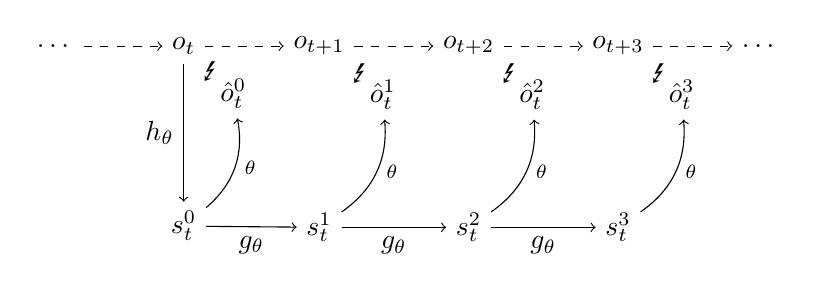
\begin{tikzpicture}[node distance=1.0]
            \node (ot) {$o_t$};
            \node [left = of ot] (otm1) {$\dots$};
            \node [right = of ot] (otp1) {$o_{t+1}$};
            \node [right = of otp1] (otp2) {$o_{t+2}$};
            \node [right = of otp2] (otp3) {$o_{t+3}$};
            \node [right = of otp3] (otp4) {$\dots$};
            \draw [->, dashed] (otm1) -- (ot);
            \draw [->, dashed] (ot) -- (otp1);
            \draw [->, dashed] (otp1) -- (otp2);
            \draw [->, dashed] (otp2) -- (otp3);
            \draw [->, dashed] (otp3) -- (otp4);

            \node [below = 1.75 of ot] (s0) {$s^0_t$};
            \node [below = 1.75 of otp1] (s1) {$s^1_t$};
            \node [below = 1.75 of otp2] (s2) {$s^2_t$};
            \node [below = 1.75 of otp3] (s3) {$s^3_t$};
            \draw [->] (ot) -- node [left] {$h_\theta$} (s0);
            \draw [->] (s0) -- node [below] {$g_\theta$} (s1);
            \draw [->] (s1) -- node [below] {$g_\theta$} (s2);
            \draw [->] (s2) -- node [below] {$g_\theta$} (s3);

            \pause

            \node [below right = 0.1 of ot] (notot) {$\hat{o}^0_t$};
            \draw [->] (s0) edge [bend right] node [right] {$\reconstruction_\theta$} (notot);
            \node [below right = -0.2 of ot] {\Lightning};

            \pause

            \node [below right = 0.1 of otp1] (nototp1) {$\hat{o}^1_t$};
            \node [below right = 0.1 of otp2] (nototp2) {$\hat{o}^2_t$};
            \node [below right = 0.1 of otp3] (nototp3) {$\hat{o}^3_t$};

            \draw [->] (s1) edge [bend right] node [right] {$\reconstruction_\theta$} (nototp1);
            \draw [->] (s2) edge [bend right] node [right] {$\reconstruction_\theta$} (nototp2);
            \draw [->] (s3) edge [bend right] node [right] {$\reconstruction_\theta$} (nototp3);

            \node [below right = -0.2 of otp1] {\Lightning};
            \node [below right = -0.2 of otp2] {\Lightning};
            \node [below right = -0.2 of otp3] {\Lightning};
        \end{tikzpicture}
        \caption{The reconstruction function $\reconstruction_\theta$ being used to predict future observations $o_{t+k}$ from internal states $s^k$ with the help of the representation function $h_\theta$ as well as the dynamics function $g_\theta$.}
        \label{fig:reconstruction_function}
    \end{figure}
\end{frame}

\subsection{Consistency Loss}

\begin{frame}[fragile]{Consistency Loss}
    \begin{figure}
        \centering
        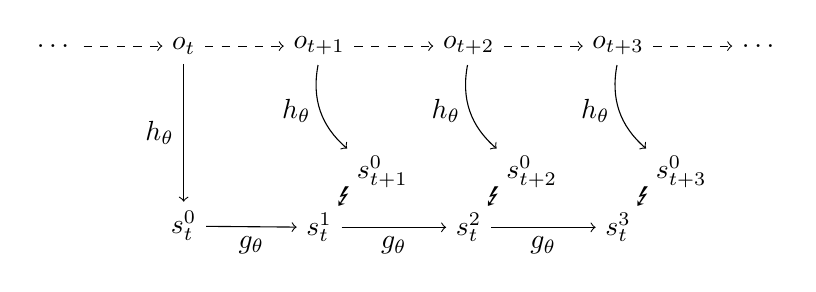
\begin{tikzpicture}[node distance=1.0]
            \node (ot) {$o_t$};
            \node [left = of ot] (otm1) {$\dots$};
            \node [right = of ot] (otp1) {$o_{t+1}$};
            \node [right = of otp1] (otp2) {$o_{t+2}$};
            \node [right = of otp2] (otp3) {$o_{t+3}$};
            \node [right = of otp3] (otp4) {$\dots$};
            \draw [->, dashed] (otm1) -- (ot);
            \draw [->, dashed] (ot) -- (otp1);
            \draw [->, dashed] (otp1) -- (otp2);
            \draw [->, dashed] (otp2) -- (otp3);
            \draw [->, dashed] (otp3) -- (otp4);

            \pause

            \node [below = 1.75 of ot] (s0) {$s^0_t$};
            \draw [->] (ot) -- node [left] {$h_\theta$} (s0);

            \pause

            \node [below = 1.75 of otp1] (s1) {$s^1_t$};
            \draw [->] (s0) -- node [below] {$g_\theta$} (s1);

            \pause

            \node [above right = 0.1 of s1] (nots1) {$s^0_{t+1}$};
            \node [above right = -0.25 of s1] {\Lightning};
            \draw [->] (otp1) edge [bend right] node [left] {$h_\theta$} (nots1);

            \pause

            \node [below = 1.75 of otp2] (s2) {$s^2_t$};
            \node [below = 1.75 of otp3] (s3) {$s^3_t$};

            \draw [->] (s1) -- node [below] {$g_\theta$} (s2);
            \draw [->] (s2) -- node [below] {$g_\theta$} (s3);

            \node [above right = 0.1 of s2] (nots2) {$s^0_{t+2}$};
            \node [above right = -0.25 of s2] {\Lightning};
            \node [above right = 0.1 of s3] (nots3) {$s^0_{t+3}$};
            \node [above right = -0.25 of s3] {\Lightning};

            \draw [->] (otp2) edge [bend right] node [left] {$h_\theta$} (nots2);
            \draw [->] (otp3) edge [bend right] node [left] {$h_\theta$} (nots3);
        \end{tikzpicture}
        \caption{Visualization of the discrepancy between state outputs of the dynamics function $g_\theta$ and representation function $h_\theta$.}
        \label{fig:consistency_loss}
    \end{figure}
\end{frame}

\newpage
\section{Experiments}
We will now perform several experiments to test and ideally validate our hypothesis that the proposed methods improve the performance of the MuZero algorithm.

Note that, in artificial intelligence research, training processes are stochastic, meaning we need to repeat experiments many times to get statistically significant results. Furthermore, in reinforcement learning in particular, the algorithms are often fragile and highly sensitive to hyperparameter changes. Errors in the implementation are sometimes difficult to find or even notice, given that their impact on the algorithm's performance may be minor.

\subsection{Environments}
For our experiments, we choose environments provided by \textit{OpenAI Gym} \cite{gym}, which is a toolkit for developing and comparing reinforcement learning algorithms. It provides us with a simple and easy to use environment interface and a wide range of environments to develop general purpose agents.

More specifically, we choose two environments, namely \textit{CartPole-v1} and \textit{LunarLander-v2}, shown in figure \ref{fig:environments}. These environments are relatively iconic in the reinforcement learning community, and, due to their simplicity, the learning progress and pitfalls can be easily understood by a human.
\begin{figure}[ht]
    \centering
    \begin{subfigure}{0.49\textwidth}
        \raggedleft
        \includegraphics[width=\textwidth]{assets/cartpole.jpg}
    \end{subfigure}
    \begin{subfigure}{0.5\textwidth}
        \raggedright
        \includegraphics[width=\textwidth]{assets/lunarlander.jpg}
    \end{subfigure}
    \caption{Screenshots of the CartPole-v1 (left) and LunarLander-v2 (right) OpenAI Gym environments.}
    \label{fig:environments}
\end{figure}
A more meaningful benchmark would include significiantly more complex environments, such as Chess and Go, as well as Atari games, as was done for the original MuZero agent. Furthermore, experiments with a robot agents, like a robotic arm grasping for objects, could provide real world applications for the algorithms. Unfortunately, due to MuZero's high computational requirements, we are unable to properly test these environments with various hyperparameters and achieve sufficient statistical significance. The exploration of more demanding environments is therefore left to future work.

In CartPole-v1, the agent controls a cart that can only move horizontally on one axis. Attached to the cart is a pole that starts off relatively upright and can freely spin around the axis perpendicular to the cart's movement. The goal is to balance the pole as long as possible such that it never exceeds $15$ degrees from being vertical. Moving the cart too far to the left or right (i.e. out of bounds) also results in episode termination. Only two actions are available, namely the acceleration in either direction, and a reward of $1$ is given for each survived timestep, up to a maximum of $500$ steps.

The objective in the LunarLander-v2 environment is, as the name suggests, to savely land a lander on the moon's surface. This is done by controlling three thrusters: A main engine, and two orientation thrusters. Various rewards are given to incentivize the agent to pursue this behavior, such as a bonus for approaching the landing pad, and a small negative penalty for using the main engine, encouraging fuel efficiency. Perhaps most notably however, a large negative reward of $-100$ is given for crashing the lander.
\subsection{Setup}
We adopt \textit{muzero-general} \cite{muzero-general}, an open source implementation of MuZero that is written in the Python programming language and uses PyTorch for automatic differentiation, as our baselines agent.
\begin{figure}[ht]
    \centering
    \tikzset{%
        cascaded/.style = {%
            general shadow = {%
            shadow scale = 1,
            shadow xshift = -1ex,
            shadow yshift = -1ex,
            draw,
            thick,
            fill = white},
            general shadow = {%
            shadow scale = 1,
            shadow xshift = -.5ex,
            shadow yshift = -.5ex,
            draw,
            thick,
            fill = white},
            fill = white, 
            draw,
            thick,
        }
    }
    \begin{tikzpicture}[every node/.style={inner sep=0.3cm}]
        \node [draw, rectangle] (reanalyze) {Reanalyze};
        \node [draw, rectangle, below = of reanalyze] (replay) {Replay Buffer};
        \node [draw, rectangle, below = 1.5cm of replay] (storage) {Shared Storage};
        \node [draw, rectangle, left = 2.5cm of storage] (trainer) {Trainer};
        \node [draw, rectangle, cascaded, right = 2.5cm of storage] (play) {Self Play};
        \node [draw, rectangle, below = 1.5cm of storage] (tensorboard) {TensorBoard};

        \draw [->] (reanalyze) edge [bend right] node[left] {update game history} (replay);
        \draw [->] (replay) edge [bend right] node[right] {sample game history} (reanalyze);

        \draw [->] (trainer) -- node[below right=-0.2cm] {update priorities} (replay);
        \draw [->] (replay) edge [bend right] node[above left] {get batch} (trainer);
        \draw [->] (trainer) -- node[below] {set weights} (storage);
        \draw [->] (storage) -- node[below] {get weights} (play);
        \draw [->] (play) -- node[above right] {save game history} (replay);

        \draw [->] (storage) -- node[left] {get info} (tensorboard);
    \end{tikzpicture}
    \caption{The parallelized worker structure of muzero-general.}
    \label{fig:muzero_general}
\end{figure}
It is heavily parallelized by employing a worker architecture (see figure \ref{fig:muzero_general}), with each worker being a seperate process that communicates with its peers through message passing. This allows for flexible scaling, even across multiple machines. Worker types include
\begin{itemize}
    \item a \textit{Replay Buffer} worker, responsible for storing game histories as experience for the learning process,
    \item a \textit{Shared Storage} worker, which holds logging information and distributes neural network weights,
    \item at least one, but potentially many \textit{Self Play} processes, each interacting with its own instance of the environment, collecting experience and filling the replay buffer,
    \item a \textit{Trainer}, which uses stored experience to perform gradient descent on the loss function, thereby improving the model,
    \item the \textit{Reanalyze} worker, responsible for continuously updating outdated search policies and values within the replay buffer and
    \item the main process, which takes logging information from the Shared Storage and outputs it to \textit{TensorBoard}, a tool that allows for live visualization of the training process.
\end{itemize}
Note that the term \textit{self-play} originates from AlphaZero or MuZero agents playing a board game like Chess against themselves to learn strategies without any human influence. Nevertheless, we use the term even for environments operated by only a single player, such as LunarLander-v2.

We modify the source code of muzero-general to include a reconstruction function and additional loss terms. The readout of the replay buffer must also be tweaked to include not only the observation at timestep $t$, but the $K$ subsequent observations $o_{t+1}, ..., o_{t+K}$ as well, as they are critical for calculating our new loss values.

The neural networks making up each of the four MuZero functions follow a very simple structure in our experiments. They consist of simple two-layer fully connected perceptrons. The first (\textit{hidden}) layer contains 16 neurons in the case of of CartPole-v1, and 64 for LunarLander-v2. The number of neurons in the second layer is determined by the desired output dimensionality. For example, the representation function must output an internal state, which, for CartPole-v1, is an eight-dimensional vector. It is therefore made up of eight neurons.

A variety of different weights are tested for each of the two loss terms in order to gauge their potential capability of improving performance, both individually and in union. Furthermore, as a means of showcasing self-supervised learning for MuZero, we pretrain a hybrid agent, that is, an agent using both modifications at the same time, for $5000$ training steps, using only the newly added loss terms, instead of the full loss formula.

Table \ref{tab:hyperparameters} shows the hyperparameters used by all tested model configurations. Most of the listed hyperparameters were kept as is from the muzero-general defaults. Note that we are unable to perform a comprehensive hyperparameter search due to technical limitations.
\begin{table}[ht]
    \centering
    \begin{tabular}{|c|l||c|c|}
        \hline
        & & CartPole-v1 & LunarLander-v2 \\
        \hline\hline

        & Training steps & 10000 & 30000 \\
        \cline{2-4}
        & Discount factor ($\gamma$) & 0.997 & 0.999 \\
        \cline{2-4}
        & TD steps ($n$) & 50 & 30 \\
        \cline{2-4}
        & Unroll steps ($K$) & 10 & 10 \\
        \cline{2-4}
        & Internal state dimensions & 8 & 10 \\
        \cline{2-4}
        & MuZero Reanalyze & Enabled & Enabled \\

        \hline

        \multirow{4.1}{*}{\begin{sideways}Losses\end{sideways}} & Optimizer & Adam & Adam \\
        \cline{2-4}
        & Learning rate ($\beta$) & $0.02 \times 0.9^{t \times 0.001}$ & 0.005 \\
        \cline{2-4}
        & Value loss weight & 1.0 & 1.0 \\
        \cline{2-4}
        & L2 regularization weight & $10^{-4}$ & $10^{-4}$ \\

        \hline

        \multirow{3.2}{*}{\begin{sideways}Replay\end{sideways}} & Replay buffer size & 500 & 2000 \\
        \cline{2-4}
        & Prioritization exponent & 0.5 & 0.5 \\
        \cline{2-4}
        & Batch size & 128 & 64 \\

        \hline

        \multirow{7.5}{*}{\begin{sideways}MCTS\end{sideways}} & Simulations & 50 & 50 \\
        \cline{2-4}
        & Dirichlet $\alpha$ & 0.25 & 0.25 \\
        \cline{2-4}
        & Exploration factor & 0.25 & 0.25 \\
        \cline{2-4}
        & pUCT $c_1$ & 1.25 & 1.25 \\
        \cline{2-4}
        & pUCT $c_2$ & 19652 & 19652 \\
        \cline{2-4}
        & Softmax temperature ($T$) & \makecell{
            1.0 if $t<5000$, \\ 0.5 if $5000 \leq t < 7500$, \\ 0.25 if $t \geq 7500$
        } & 0.35 \\

        \hline
    \end{tabular}
    \caption{Hyperparameter selection for all tested agents. Parameters based on the current training step use the variable $t$.}
    \label{tab:hyperparameters}
\end{table}

 Performance is measured by training an agent for a specific amount of training steps and, at various time steps, sampling the total episode reward the agent can achieve.

\subsection{Results}

\begin{frame}[fragile]{Reconstruction Function}
    \begin{figure}
        \centering
        \begin{tikzpicture}[yscale=0.6, xscale=0.6,
                            define rgb/.code={\definecolor{mycolor}{RGB}{#1}},
                            rgb color/.style={define rgb={#1},mycolor}]
            \begin{axis}[
                title = CartPole-v1,
                axis lines = left,
                xlabel = Training steps,
                ylabel = Total reward,
                no markers,
                table/col sep = comma,
                legend cell align=left,
                legend pos=south east,
                legend style={draw=none},
                xmin=0,
                xmax=10000,
                grid=major,
            ]
                \addplot[black] table [
                    x = training_step,
                    y = reward,
                ] {results/default/CartPole-v1/lr0.0.csv};
                \addlegendentry{MuZero};

                \addplot[rgb color={32, 32, 180}] table [
                    x = training_step,
                    y = reward,
                ] {results/reconstruction/CartPole-v1/lr0.5.csv};
                \addlegendentry{$\frac{1}{2}l^g$};

                \addplot[rgb color={128, 128, 255}] table [
                    x = training_step,
                    y = reward,
                ] {results/reconstruction/CartPole-v1/lr1.0.csv};
                \addlegendentry{$l^g$};
            \end{axis}
        \end{tikzpicture}
        \begin{tikzpicture}[yscale=0.6, xscale=0.6,
                            define rgb/.code={\definecolor{mycolor}{RGB}{#1}},
                            rgb color/.style={define rgb={#1},mycolor}]
            \begin{axis}[
                title = LunarLander-v2,
                axis lines = left,
                xlabel = Training steps,
                ylabel = Total reward,
                no markers,
                table/col sep = comma,
                legend cell align=left,
                legend pos=south east,
                legend style={draw=none},
                xmin=0,
                xmax=30000,
                grid=major,
            ]
                \addplot[black] table [
                    x = training_step,
                    y = reward,
                ] {results/default/LunarLander-v2/lr0.0.csv};
                \addlegendentry{MuZero};

                \addplot[rgb color={32, 32, 180}] table [
                    x = training_step,
                    y = reward,
                ] {results/reconstruction/LunarLander-v2/lr0.5.csv};
                \addlegendentry{$\frac{1}{2}l^g$};

                \addplot[rgb color={128, 128, 255}] table [
                    x = training_step,
                    y = reward,
                ] {results/reconstruction/LunarLander-v2/lr1.0.csv};
                \addlegendentry{$l^g$};
            \end{axis}
        \end{tikzpicture}
        \caption{Total episode reward comparison of agents using the reconstruction loss term ($l^g$) and the default MuZero agent in the CartPole-v1 and LunarLander-v2 environments, averaged across 32 and 25 runs, respectively.}
        \label{fig:reconstruction_results}
    \end{figure}
\end{frame}

\begin{frame}[fragile]{Consistency Loss}
    \begin{figure}
        \centering
        \begin{tikzpicture}[yscale=0.6, xscale=0.6,
                            define rgb/.code={\definecolor{mycolor}{RGB}{#1}},
                            rgb color/.style={define rgb={#1},mycolor}]
            \begin{axis}[
                title = CartPole-v1,
                axis lines = left,
                xlabel = Training steps,
                ylabel = Total reward,
                no markers,
                table/col sep = comma,
                legend cell align=left,
                legend pos=south east,
                legend style={draw=none},
                xmin=0,
                xmax=10000,
                grid=major,
            ]
                \addplot[black] table [
                    x = training_step,
                    y = reward,
                ] {results/default/CartPole-v1/lr0.0.csv};
                \addlegendentry{MuZero};

                \addplot[rgb color={32, 128, 32}] table [
                    x = training_step,
                    y = reward,
                ] {results/consistency/CartPole-v1/lr0.5.csv};
                \addlegendentry{$\frac{1}{2}l^c$};

                \addplot[rgb color={0, 255, 0}] table [
                    x = training_step,
                    y = reward,
                ] {results/consistency/CartPole-v1/lr1.0.csv};
                \addlegendentry{$l^c$};
            \end{axis}
        \end{tikzpicture}
        \begin{tikzpicture}[yscale=0.6, xscale=0.6,
                            define rgb/.code={\definecolor{mycolor}{RGB}{#1}},
                            rgb color/.style={define rgb={#1},mycolor}]
            \begin{axis}[
                title = LunarLander-v2,
                axis lines = left,
                xlabel = Training steps,
                ylabel = Total reward,
                no markers,
                table/col sep = comma,
                legend cell align=left,
                legend pos=south east,
                legend style={draw=none},
                xmin=0,
                xmax=30000,
                grid=major,
            ]
                \addplot[black] table [
                    x = training_step,
                    y = reward,
                ] {results/default/LunarLander-v2/lr0.0.csv};
                \addlegendentry{MuZero};

                \addplot[rgb color={32, 128, 32}] table [
                    x = training_step,
                    y = reward,
                ] {results/consistency/LunarLander-v2/lr0.5.csv};
                \addlegendentry{$\frac{1}{2}l^c$};

                \addplot[rgb color={0, 255, 0}] table [
                    x = training_step,
                    y = reward,
                ] {results/consistency/LunarLander-v2/lr1.0.csv};
                \addlegendentry{$l^c$};
            \end{axis}
        \end{tikzpicture}
        \caption{Total episode reward comparison of agents the consistency loss ($l^c$) and the default MuZero agent in the CartPole-v1 and LunarLander-v2 environments, averaged across 32 and 25 runs, respectively.}
        \label{fig:consistency_results}
    \end{figure}
\end{frame}

\begin{frame}[fragile]{Hybrid Method}
    \begin{figure}
        \centering
        \begin{tikzpicture}[yscale=0.6, xscale=0.6,
                            define rgb/.code={\definecolor{mycolor}{RGB}{#1}},
                            rgb color/.style={define rgb={#1},mycolor}]
            \begin{axis}[
                title = CartPole-v1,
                axis lines = left,
                xlabel = Training steps,
                ylabel = Total reward,
                no markers,
                table/col sep = comma,
                legend cell align=left,
                legend pos=south east,
                legend style={draw=none},
                xmin=0,
                xmax=10000,
                grid=major,
            ]
                \addplot[black] table [
                    x = training_step,
                    y = reward,
                ] {results/default/CartPole-v1/lr0.0.csv};
                \addlegendentry{MuZero};

                \addplot[rgb color={128, 128, 255}] table [
                    x = training_step,
                    y = reward,
                ] {results/reconstruction/CartPole-v1/lr1.0.csv};
                \addlegendentry{$l^g$};

                \addplot[rgb color={0, 128, 128}] table [
                    x = training_step,
                    y = reward,
                ] {results/hybrid/CartPole-v1/lr0.5.csv};
                \addlegendentry{$\frac{1}{2}l^g + \frac{1}{2}l^c$};

                \addplot[rgb color={0, 200, 200}] table [
                    x = training_step,
                    y = reward,
                ] {results/hybrid/CartPole-v1/lr1.0.csv};
                \addlegendentry{$l^g + l^c$};
            \end{axis}
        \end{tikzpicture}
        \begin{tikzpicture}[yscale=0.6, xscale=0.6,
                            define rgb/.code={\definecolor{mycolor}{RGB}{#1}},
                            rgb color/.style={define rgb={#1},mycolor}]
            \begin{axis}[
                title = LunarLander-v2,
                axis lines = left,
                xlabel = Training steps,
                ylabel = Total reward,
                no markers,
                table/col sep = comma,
                legend cell align=left,
                legend pos=south east,
                legend style={draw=none},
                xmin=0,
                xmax=30000,
                grid=major,
            ]
                \addplot[black] table [
                    x = training_step,
                    y = reward,
                ] {results/default/LunarLander-v2/lr0.0.csv};
                \addlegendentry{MuZero};

                \addplot[rgb color={128, 128, 255}] table [
                    x = training_step,
                    y = reward,
                ] {results/reconstruction/LunarLander-v2/lr1.0.csv};
                \addlegendentry{$l^g$};

                \addplot[rgb color={0, 128, 128}] table [
                    x = training_step,
                    y = reward,
                ] {results/hybrid/LunarLander-v2/lr0.5.csv};
                \addlegendentry{$\frac{1}{2}l^g + \frac{1}{2}l^c$};

                \addplot[rgb color={0, 200, 200}] table [
                    x = training_step,
                    y = reward,
                ] {results/hybrid/LunarLander-v2/lr1.0.csv};
                \addlegendentry{$l^g + l^c$};
            \end{axis}
        \end{tikzpicture}
        \caption{Total episode reward comparison of agents using both the reconstruction function loss ($l^g$) as well as the consistency loss term ($l^c$) simultaneously in the CartPole-v1 and LunarLander-v2 environments, averaged across 32 and 25 runs, respectively.}
        \label{fig:hybrid_results}
    \end{figure}
\end{frame}

\begin{frame}[fragile]{Pretrained Hybrid}
    \begin{figure}
        \centering
        \begin{tikzpicture}[yscale=0.6, xscale=0.6,
                            define rgb/.code={\definecolor{mycolor}{RGB}{#1}},
                            rgb color/.style={define rgb={#1},mycolor}]
            \begin{axis}[
                title = CartPole-v1,
                axis lines = left,
                xlabel = Training steps,
                ylabel = Total reward,
                no markers,
                table/col sep = comma,
                legend cell align=left,
                legend pos=south east,
                legend style={draw=none},
                xmin=0,
                xmax=10000,
                grid=major,
            ]
                \addplot[black] table [
                    x = training_step,
                    y = reward,
                ] {results/default/CartPole-v1/lr0.0.csv};
                \addlegendentry{MuZero};

                \addplot[rgb color={0, 200, 200}] table [
                    x = training_step,
                    y = reward,
                ] {results/hybrid/CartPole-v1/lr1.0.csv};
                \addlegendentry{$l^g + l^c$};

                \addplot[rgb color={220, 80, 80}] table [
                    x = training_step,
                    y = reward,
                ] {results/pretrained/CartPole-v1/lr1.0.csv};
                \addlegendentry{$l^g + l^c$ (pretrained)};
            \end{axis}
        \end{tikzpicture}
        \begin{tikzpicture}[yscale=0.6, xscale=0.6,
                            define rgb/.code={\definecolor{mycolor}{RGB}{#1}},
                            rgb color/.style={define rgb={#1},mycolor}]
            \begin{axis}[
                title = LunarLander-v2,
                axis lines = left,
                xlabel = Training steps,
                ylabel = Total reward,
                no markers,
                table/col sep = comma,
                legend cell align=left,
                legend pos=south east,
                legend style={draw=none},
                xmin=0,
                xmax=30000,
                grid=major,
            ]
                \addplot[black] table [
                    x = training_step,
                    y = reward,
                ] {results/default/LunarLander-v2/lr0.0.csv};
                \addlegendentry{MuZero};

                \addplot[rgb color={0, 200, 200}] table [
                    x = training_step,
                    y = reward,
                ] {results/hybrid/LunarLander-v2/lr1.0.csv};
                \addlegendentry{$l^g + l^c$};

                \addplot[rgb color={220, 80, 80}] table [
                    x = training_step,
                    y = reward,
                ] {results/pretrained/LunarLander-v2/lr1.0.csv};
                \addlegendentry{$l^g + l^c$ (pretrained)};
            \end{axis}
        \end{tikzpicture}
        \caption{Total episode reward comparison of agents using both the reconstruction function loss ($l^g$) as well as the consistency loss term ($l^c$) simultaneously as a pretrained and non-pretrained variant in the CartPole-v1 and LunarLander-v2 environments, averaged across 32 and 25 runs, respectively.}
        \label{fig:pretrained_results}
    \end{figure}
\end{frame}
\subsection{Discussion}
The results show that all modified agents we tested exceed the performance of the unchanged MuZero agent on all environments, some, especially the agents including both proposed changes simultaneously, by a large amount. The reconstruction function seems to be the more influential of the two changes, given that it achieved a bigger performance increase than the consistency loss, and comes very close to even the hybrid agent. Even so, the consistency loss has the advantage of being simpler in its implementation by not requiring a fourth function, potentially made up of complex neural networks requiring maintenance by experts, to be added.

Agents that were pretrained in a self-supervised fashion ahead of time performed very well in the early stages of training but were unable to outmatch their fully trained counterparts. This is to be expected. While self-supervised pretraining is meant to accelerate learning, there is no argument as to why training with partial information should yield higher maximum scores in the long run. In CartPole-v1, the pretrained agent was even significantly worse than the non-pretrained version after roughly $1000$ training steps. This is likely due to the parameters and internal state representations of the model prematurely converging, to some extent, to a local minimum, which made reward and value estimations more difficult after the goal was introduced. The use of L2 regularization during pretraining may prevent this unwanted convergence.

It is still unclear whether the consistency loss provides additional value to the algorithm that is not reproducible by the reconstruction loss. While the excellent performance of the hybrid agent does suggest a benefit, we may see similar results when further increasing the weight of the reconstruction loss, considering that the agent using the highest tested loss weight performed the best. This would render the hybrid architecture unnecessary. Thus, further investigation regarding hyperparameter choices is required.

While the consistency loss resulted in a performance increase, the experiments were not designed to confirm that state representations did indeed become more consistent. Future work should also validate our hypothesis stating that the consistency loss may lessen the accuracy falloff when planning further than $K$ timesteps into the future, with $K$ being the number of unrolled steps during training.


\newpage
\section{Conclusion}

\newpage

\bibliography{bibliography}
\bibliographystyle{apalike}

\end{document}